\chapter{Evaluation}
\label{chap:evaluation}

The presented map-merging algorithm (chapter~\ref{chap:mergingalgorithm}) has been evaluated on number of demanding robotics datasets. The datasets include data captured by small aerial vehicles (sections~\ref{sec:euroc-dataset}, \ref{sec:aau-dataset}) as well as ground-based robots. The datasets include both widely used benchmark datasets in robotics research as well as data recorded by the author.

Sensors used include stereo rig cameras, active \gls{RGB-D} cameras and laser scans? This variety of sensors and robots covers many typical multi-robot deployments. All datasets has been captured under real-word conditions, none of them uses simulated data.

The evaluation focuses on properties of the presented pair-wise transformation estimation algorithm for pointclouds (section~\ref{sec:estimate-pair-wise}, which is the core algorithm of the map-merging \gls{ROS} node (section~\ref{sec:ros-package}. Accuracy of the estimation algorithm is critical for the overall map-merging process.

\section{The EuRoC micro aerial vehicle datasets}
\label{sec:euroc-dataset}

The dataset introduced by~\citet{Burri2016} was collected on-board a micro aerial vehicle equipped with stereo camera rig and \gls{IMU}. Calibration data for the cameras and ground-truth data are provided with the dataset. This dataset has been used extensively for evaluation of the visual \gls{SLAM} algorithms and visual odometry approaches.

The cameras produce a WVGA monochrome (greyscale) images at $20$ frames per second. Cameras have a global shutter. The automatic exposure control is independent for both cameras. According to the published errata~\citep{Burri2016}, this resulted in different shutter times and in turn in different image brightnesses, rendering stereo matching and feature tracking more challenging.

The dataset contains $11$ mapping sessions in $3$ different environments. Each mapping session is available in a single \gls{ROS} bag file. First $5$ sessions were captured in ETH machine hall (figure~\ref{fig:eth-machine-hall}), a fairly large industrial environment featuring piping, reservoirs and many different types of surfaces. Second and third batch of datasets were captured in a smaller furnished rectangular room. For the second and the third batch the furnishing was different.

\begin{figure}
    \centering
    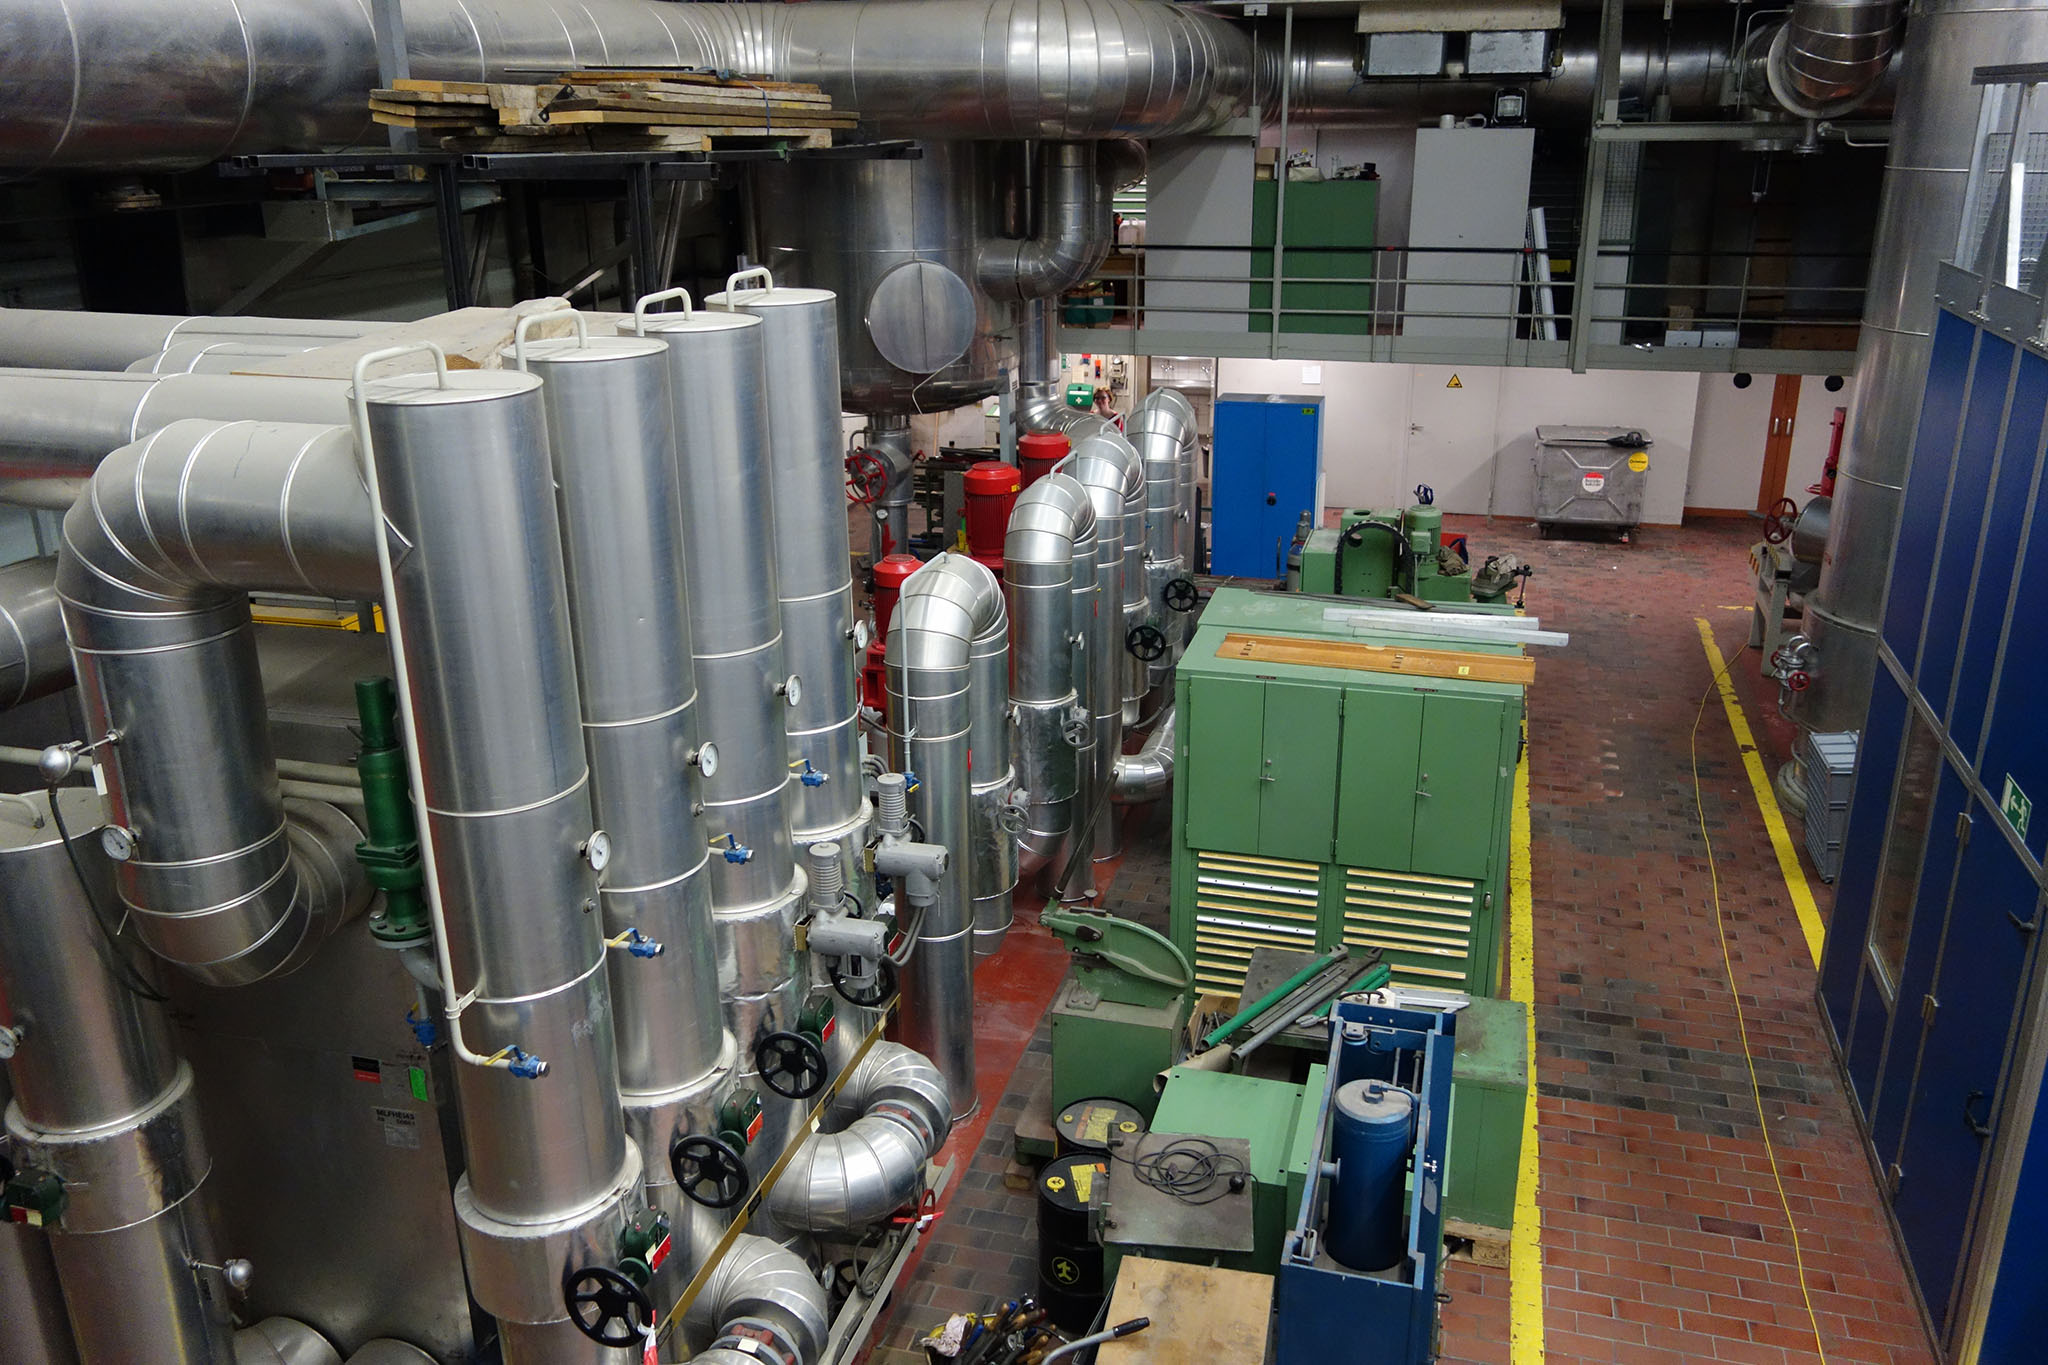
\includegraphics[width=\textwidth]{../img/eth_machine_room.jpg}
    \caption[ETH Machine hall]{ETH Machine hall industrial environment where $5$ mapping sessions of EuRoC dataset were captured. The image is courtesy of the authors~\citep{Burri2016}.}
    \label{fig:eth-machine-hall}
\end{figure}

The dataset is intended for evaluating \gls{SLAM} algorithms, for our purposes it was necessary to process the data with a \gls{SLAM} algorithm to create a pointcloud maps. First, I have used the provided calibration sequence and I have created a calibration data for \gls{ROS} using the \texttt{camera\_calibration} tool available with \gls{ROS}.

Second, for each environment I created a pair of maps using the $01$ and $02$ mapping sessions from the datasets, which were used further for the evaluation of the map-merging. I used a RTAB-Map \gls{SLAM}, developed by~\citet{labbe2014online}, to create the maps. The odometry for mapping was provided from stereo camera data, using a visual odometry approach, the available \gls{IMU} data were not used.

% finish diffucult maps, articats, differnt visual odometry

% todo add maps figures

\section{AAU dataset}
\label{sec:aau-dataset}

\section{MFF dataset}
\label{sec:mff-dataset}